\section{Validation}
The extent to which the technique serves it purpose is defined by its soundness, efficiency and, more importantly, information, the latter understood as the ability to guide the engineer while writing a non trivial formal specification. The presented diagnosis should help by pointing out the causes of non realizability, expressed in a language where the behavior of the plant, or as in this case a part of it, is explicit. The diagnosis tool set should be a part of the specification process and must be present while progressively gathering knowledge and refining the model towards its intended form.

The measure of information our technique provides must be related to the impact it can have on the overall specification process, in particular in how clear it is for the engineer  to interpret the diagnosis. The aim is to minimize the amount of data presented while keeping it relevant to the non realizability cause. The unavailability of skilled professionals and the amount of time and effort required to prepare a considerable set of external subjects up to the point where they would be able to write non trivial formal specifications, renders the perspective of a controlled experiment with external engineers writing specifications from scratch unfeasible. On the other hand, it is also impossible to propose a direct comparison with similar techniques, since, for instance, in ~\cite{DBLP:conf/hvc/KonighoferHB10} the minimization is applied on the set of environmental safety formulas, which in fact increments the volume of the plant when presented as an automaton, and in ~\cite{DBLP:conf/sigsoft/KuventMR17} a simplification of the symbolic counter strategy is presented as a LTS composed of attractors and trap states. We think that our technique adds a complimentary view to the non realizability diagnosis problem.

We now explain two of the metrics used to quantitatively evaluate our technique. The first metric is relative minimization volume ($v_{\mathcal{U}}$), defined as the size of the minimized plant against the original instance ($|\Delta_{E'}|/|\Delta_{E}|$). 
The number of transitions is used as the representation of absolute volume for two reasons, first, because it is a measure of how many options the user has when exploring the minimized plant, and the  and second, because it is the defining parameter in the complexity of the synthesis algorithms. 
The other metric we compute is minimization volume relative to the controller volume ($v_{\mathcal{C}}=|\Delta_{E'}|/|\Delta_{C}|$). The controller $C$ is the automaton representation of the strategy for the realizable version of each specification. The rationale behind this is that the size of the controller is a good proxy for the volume of the engineer's design intent in terms of concrete behavior. The motivation for taking the controller as a proxy of volume is that sometimes an ongoing specification is under defined, with weaker conditions than it will eventually have when reaching realizability. We expect our minimization to be at least comparable to the controller in terms of volume.

The validation reported in this section is guided by two main concerns.  This first is the degree to which the initial control problem is reduced and the computational cost involved. The second is if the minimization offers insight into non realizability causes.
In order to avoid bias, we prioritized using non realizable specifications present in the existing benchmarks and literature.

%refs 
For the test cases we first wrote and synthesized the realizable version for each instance, and then modified it
to violate at least one of the original guarantees. 
These modifications are of two different kind, the first removes a required liveness assumptions from the original specification, the second relaxes a part of the environment by removing a safety environmental constraint. Both modifications capture the way in wich a model evolves, the liveness omission stands for those situations where the environment is being mined for assumptions, which is both a partial and progressive process. The safety modification stands for those scenarios where the engineer is trying to figure out the explicit behavior of the plant, either by logically restricting the formula that describes it, or by defining and removing explicit transitions in the process-oriented syntax, in both cases non realizability is introduced by constraining the system or relaxing the environment. We restrict ourselves to missing liveness assumptions under the premise that it is usually the case that the user has a clear intent of what the system should achieve (liveness guarantees) but needs to gain knowledge of the environment in which it will operate.  Because of this we are not considering the cases where non realizability is due to the fact of the guarantees being too strong. We are presenting only one variation per case since, in the parameterized examples, most of the liveness modifications produce symmetrical diagnosis. Our approach follows Cimatti's ~\cite{DBLP:conf/vmcai/CimattiRST08} in creating minimaly unfulfillable conflict by removing the smaller set of liveness assumptions to achieve non realizability.
 
We will now briefly explain each case, show how the they were parameterized and modified in order to achieve non realizability. The Generalized Buffer (GenBuf) and AMBA AHB case studies were taken from~\cite{DBLP:conf/hvc/KonighoferHB10}, the Lift Controller comes from ~\cite{DBLP:conf/fmcad/AlurMT13}, Collector is part of the SYNTCOMP competition ~\cite{SYNTCOMP} benchmark and the exploration robot case was adapted from ~\cite{DBLP:journals/corr/abs-2001-07678}. 
%lift controller
The \textbf{Lift Controller} case specifies the behavior of a system that should eventually serve every request to take the elevator to a required floor when the corresponding button was pressed, and also to take it back to the ground floor if no request is pending. The parameter on these instances indicates how many floors are present in the specification. The \texttt{missing liveness} modification changes one of the liveness guarantees from $\square \Diamond (b_i \rightarrow f_i)$ to $\square \Diamond (f_i)$. The original form asks the system to serve a floor only when requested, the modification makes it serve a floor even when it was not requested. Due to other safety restrictions this renders the specification unrealizable. The \texttt{removed safety} modification allows an input signal to keep the elevator at a particular floor indefinitely.

%collector
The \textbf{Collector} case outputs a barrier signal once all inputs $in_1\ldots in_n$ have occurred at least once. The parameter indicates how many inputs the specification could receive. The \texttt{missing liveness} modification removes one of the assumptions that forces the environment to always eventually produce input $i$ ($\square\Diamond(in_i)$). The \texttt{removed safety} modification removes the relation between an input and an internal memory signal that is needed in order to keep track of the inputs read after the last barrier raise.

%exploration robot
The \textbf{Exploration Robot} case models the behavior of a robot that can move through a sqare grid of size $n$, which also serves as the parameter for this specification. The robot must load cargo at the initial position and then unload it at the opposite corner of the grid. At the loading site the operation can either be successful or fail. The \texttt{missing liveness} modification removes the assumption that a load will always eventually occur. The \texttt{removed safety} modification allows the environment to neglect the load event indefinitely once a certain point in the grid is reached.

%genbuf
The \textbf{Generalized Buffer (GenBuf)} case has a FIFO for storing data incoming from senders, and a
controller to communicate with the senders, receivers, and the
FIFO. On the sender side, GenBuf receives a request input from each sender, and replies
with an acknowledge output. On the receiver side, GenBuf outputs a request and inputs an
acknowledge for each receiver. The GenBuf controller gets the \texttt{FULL} and \texttt{EMPTY} signals from the FIFO and
provides the \texttt{ENQ,DEQ}, and \texttt{SLC} signals for writing (reading) appropriate data to (from) the FIFO.
The parameter on each instance indicates how many senders the specification has. The \texttt{missing liveness} modification removes the assumption that the first receiver will eventually acknowledge a request, and in \texttt{removed safety} we removed original assumption \texttt{A5}, relaxing the behavior of the \texttt{FULL} and \texttt{EMPTY} signals.

%ahb
The \textbf{AMBA AHB} defines a standard for on-chip communication between several devices operating in master-slave fashion. We split the arbiter in two modules, the \texttt{scheduler}, that is in charge of granting access to the masters and handling communication with the slaves, and the \texttt{burst manager}, that is in charge of handling signal burst operation. In this section we show the results for the \texttt{scheduler} since it is the only parameterized module of the two. 
The \texttt{missing liveness} modification removes the assumption that the \texttt{DECIDE} signal will always eventually be raised, which in turn does not assures that the scheduler will pick the next master to be served, and in \texttt{removed safety} the occurrence of \texttt{sel$_0$} fixes \texttt{hReq$_1$} to a low value, preventing the second master to be acknowledged. 

%tool support - tool/translation/diagnosis
The diagnosis technique was implemented in a new tool that accepts specifications expressed as both LTL formulas or FSP constructs and operates internally on CLTS structures. Each case study was written in its original syntax, for signal based specifications we used LTL formulas (as presented in ~\cite{Bloem:2012}), and for those initially described using process-like syntax we used CFSP. This tool was written from scratch with the intention to model, verify and synthesize reactive systems over explicit models in an effective fashion. Bear in mind that for each specification the diagnosis runs a number of synthesis checks (each one having its particular time complexity) linear in time in relation to the number of transitions of the original plant.
Prior to this work the only feedback given to the user  when specifying an non realizable problem over an explicit model was binary, either the problem was realizable or it was not.
he extension builds a minimized non realizable version of the environment that can then be exported to different formats and inspected through various methods including animations and visualization of the state space.

In the following we report quantitatively on all case studies to show the degree to which the initial control problem is reduced and the computational cost involved. We also briefly explain the case studies and provide an interpretation of what we think are the hints extracted from the diagnosis. 

%technical text
The quantitative results of our experiments are shown in table 
\ref{table:quantitative-results} and were run on an 
\texttt{Intel\textsuperscript{\textregistered} Core\textsuperscript{\texttrademark}
 i7-8565U} CPU with 8 processors running at 1.80GHz frequency
with 32 Gb of RAM memory over \texttt{Ubuntu 20.04 (Linux 5.4 kernel release)}.
Total time taken by the diagnosis algorithm is measured in seconds and
labeled as \emph{Diag. time(s)}, \emph{Diag. steps} shows the number of steps the diagnosis algorithm had to take to yield a minimal plant, this can be thought as de maximum depth of recursion reached while exploring the semi-lattice of alternating Sub-LTS structures.  The values in column $|\varphi_e + \varphi_s|$ are the sum of environmental and system liveness formulae, $|\Delta_{E}|$ the number of transitions in the original plant, $|\Delta_{E'}|$ the number of transitions in the minimization,
, $|\Delta_{E'}|/|\Delta_{E}|$ is the relation of the minimization volume against the original plant, , $|\Delta_{C}|$ the number of transitions in the controller for the realizable specification,
, $|\Delta_{E'}|/|\Delta_{C}|$ is the relation of the minimization volume against the controller.
We defined a timeout for each case study of 45 minutes and reported all instances below that limit.
\begin{table*}
	\resizebox{\textwidth}{!} {
% latex table generated in R 3.6.3 by xtable 1.8-4 package
% Fri Aug 14 15:17:05 2020
\begin{tabular}{|l|rr|rr|rr|rr|}
  \hline & \multicolumn{2}{c|}{Diagnosis}&\multicolumn{2}{c|}{Plant ($E$)} & \multicolumn{2}{c|}{Minimization ($v_{\mathcal{U}}$)} & \multicolumn{2}{c|}{Controller ($v_{\mathcal{C}}$)}\\ \hline
Name & Diag. time(s) & Diag. steps & $|\varphi_e + \varphi_s|$ & $|\Delta_E|$ & $|\Delta_{E'}|$ & $|\Delta_{E'}|/|\Delta_{E}|$ & $|\Delta_{C}|$ & $|\Delta_{E'}|/|\Delta_{C}|$ \\ 
  \hline
Lift Controller 2 (missing assumption) & 0.015 & 3 & 5 & 52 & 4 & 0.0769 & 116 & 0.4483 \\ 
  Lift Controller 4 (missing assumption) & 0.037 & 8 & 7 & 1088 & 4 & 0.0037 & 3238 & 0.3360 \\ 
  Lift Controller 6 (missing assumption) & 1.069 & 12 & 9 & 15720 & 4 & 0.0003 & 61400 & 0.2560 \\ 
  Lift Controller 8 (missing assumption) & 150.302 & 17 & 11 & 195040 & 20 & 0.0001 & 937004 & 0.2082 \\ 
  Collector 1 (missing assumption) & 0.003 & 4 & 2 & 39 & 4 & 0.1026 & 29 & 0.1379 \\ 
  Collector 2 (missing assumption) & 0.024 & 15 & 2 & 253 & 8 & 0.0316 & 182 & 0.0440 \\ 
  Collector 3 (missing assumption) & 0.061 & 21 & 3 & 1815 & 16 & 0.0088 & 1259 & 0.0127 \\ 
  Collector 4 (missing assumption) & 0.241 & 22 & 4 & 13621 & 18 & 0.0013 & 9305 & 0.0019 \\ 
  Collector 5 (missing assumption) & 5.158 & 48 & 5 & 104799 & 16 & 0.0002 & 71093 & 0.0002 \\ 
  Exploration Robot 12 (missing assumption) & 0.149 & 6 & 3 & 1320 & 202 & 0.1530 & 162 & 1.2469 \\ 
  Exploration Robot 15 (missing assumption) & 0.105 & 2 & 3 & 2010 & 365 & 0.1816 & 320 & 1.1406 \\ 
  Exploration Robot 18 (missing assumption) & 0.210 & 2 & 3 & 2844 & 512 & 0.1800 & 456 & 1.1228 \\ 
  Exploration Robot 21 (missing assumption) & 1.685 & 7 & 3 & 3822 & 775 & 0.2028 & 698 & 1.1103 \\ 
  Exploration Robot 24 (missing assumption) & 2.922 & 7 & 3 & 4944 & 970 & 0.1962 & 894 & 1.0850 \\ 
  Exploration Robot 27 (missing assumption) & 1.030 & 2 & 3 & 6210 & 1301 & 0.2095 & 1220 & 1.0664 \\ 
  Exploration Robot 30 (missing assumption) & 1.503 & 2 & 3 & 7620 & 1568 & 0.2058 & 1476 & 1.0623 \\ 
  Exploration Robot 6 (missing assumption) & 0.012 & 2 & 3 & 361 & 30 & 0.0831 & 174 & 0.1724 \\ 
  Exploration Robot 9 (missing assumption) & 0.041 & 6 & 3 & 774 & 116 & 0.1499 & 86 & 1.3488 \\ 
  Genbuf 1 (missing assumption) & 0.017 & 6 & 4 & 273 & 48 & 0.1758 & 307 & 0.8893 \\ 
  Genbuf 2 (missing assumption) & 2.941 & 23 & 5 & 28706 & 610 & 0.0212 & 78008 & 0.3680 \\ 
  Genbuf 3 (missing assumption) & 2593.529 & 126 & 6 & 528650 & 2539 & 0.0048 & 1918013 & 0.2756 \\ 
  Genbuf 1 (removed safety) & 0.039 & 10 & 5 & 1388 & 8 & 0.0058 & 307 & 0.0261 \\ 
  Genbuf 2 (removed safety) & 833.414 & 194 & 8 & 142850 & 834 & 0.0058 & 78008 & 0.0107 \\ 
   \hline
\end{tabular}

}
  \caption{Quantitative results for minimized plants}
  \label{table:quantitative-results}
 \end{table*}
\begin{figure}[bt]
	\centering
	\SmallPicture
	\includegraphics[width=0.3\textwidth, angle=-90]{../experimental_setting/tmp_results/size_vs_diag_time.ps}
	\vspace*{-2mm}
	\caption{Minimization size vs. diagnosis time.}
	\label{fig:size_vs_diag_time}
	\vspace*{-4mm}
	\MediumPicture
\end{figure}
%\begin{figure}[bt]
%	\centering
%	\SmallPicture
%	\includegraphics[width=0.3\textwidth, angle=-90]{../experimental_setting/tmp_results/genbuf_2_time_plot.ps}
%	\vspace*{-2mm}
%	\caption{Generic buffer (2 senders) time progression.}
%	\label{fig:genbuf_2_time_plot}
%	\vspace*{-4mm}
%	\MediumPicture
%\end{figure}
%\begin{figure}[bt]
%	\centering
%	\SmallPicture
%	\includegraphics[width=0.3\textwidth, angle=-90]{../experimental_setting/tmp_results/genbuf_2_size_plot.ps}
%	\vspace*{-2mm}
%	\caption{Generic buffer (2 senders) size progression.}
%	\label{fig:genbuf_2_size_plot}
%	\vspace*{-4mm}
%	\MediumPicture
%\end{figure}
\begin{figure}[bt]
	\centering
	\SmallPicture
	\includegraphics[width=0.3\textwidth, angle=-90]{../experimental_setting/tmp_results/min_ctrl_vs_min_pct.ps}
	\vspace*{-2mm}
	\caption{Minimization controllability vs. minimization percentage.}
	\label{fig:min_ctr_vs_min_pct}
	\vspace*{-4mm}
	\MediumPicture
\end{figure}
%update quantitative analysis and explain graphs
%table
%size

%replace this paragraph with something related to the time it takes to finish the diagnosis w.r.t. the time of synthesis in the realizable case
The results we observe after applying the technique on this initial set of case studies show the proposed approach is feasible even for a significant number of signal based specifications. 
As expected with any algorithm working with explicit models, the minimization technique still under performs against symbolic approaches on both size and time. 

%time
In figure ~\ref{fig:size_vs_diag_time} we expose the relation between diagnosis time and plant size (measured in number of initial transitions). We argue that the performance of the algorithm is linearly consistent (yielding a $\tau$ value of .76 using Kendall correlation) across the range of sizes present in the test set (going from tens to hundred of thousands of transitions). This is relevant because the synthesis procedure has a polynomial cost in terms of its input, so a polynomial increase in the cost of diagnosis in relation to its input size could be expected. 
%controllability and post processing
We also found that the amount of minimization achievable seems to be related to how controllable the result is, as expressed in figure  ~\ref{fig:min_ctr_vs_min_pct} in the number of controllable transitions in the minimization over the number of total transitions. The relation seems to be linear (yielding a $\tau$ value of .89 using Kendall correlation).
%final remarks
From the results it is possible to argue that the minimization technique can be applied to control problems of similar size to those reported in the literature. 
%In addition, it is possible to observe, as expected, that the  that spatial and temporal limitation behave linearly with respect to the realizability query. 
In addition, it can be seen that the technique can achieve a significant reduction in terms of states and transitions. Even when the reduction is significant in the bigger examples, as the 0.48\% reduction for 528650 transitions in the biggest generic buffer case, the resulting 2539 transitions are still enough to make manual inspection difficult. We assume that in this cases the technique can be used as the initial step of the diagnosis, allowing for other techniques to be applied afterwards, such as existential quantification or collapsing $\sigma$-traps.
Going back to the problem of comparing our technique to the symbolic approaches, ~\cite{DBLP:conf/hvc/KonighoferHB10} reports an average reduction of the presented formulae of a 90\% and our approach has a marginal better value of 97,8\%.

In terms of the retained behavior the initial size of the specification determines whether the minimization can be manually inspected or not, except for the Lift Controller and Collector cases. These are minimized to the point where it is easy to see that the plant never produces a particular set of signals. In the exploration robot case it is necessary to execute a short trace before reaching a loop that violates the assumption that a loads always eventually occurs. For the Genbuf case the non realizability cause is easily spotted in the initial parameter, but requires some exploration for the other numbers. We suppose that a novice user can directly benefit from the diagnosis in the most of the cases but will require an additional step involving label hiding or signal quantification for some of them to be able to promptly identify the problem.
%
%
%\subsection{Modified Lift Controller}
%Another example that has been evaluated is that
%of the Modified Lift Controller from 
%\cite{DBLP:conf/fmcad/AlurMT13} first presented in
%its realizable version in 
%\cite{DBLP:journals/jcss/BloemJPPS12}.
%In the original version a lift controller should serve
%several floors.  It has a button sensor for each floor 
%controlled by the environment.  There is an additional 
%restriction that allows the lift to move up only if there
%is a pending request in one of the floors 
%($\square \Diamond (b_j \implies f_j)$), and another that
%forces the system to visit the first floor infinitely
%often if no button was pressed.\\
%In the modified version from ~\cite{DBLP:conf/fmcad/AlurMT13} a new set of system liveness 
%requirements is added, where the system should 
%visit each floor infinitely often ($\square \Diamond f_j$).
%
%
%The problem here is that this requirement collides with
%the restriction that the lift will not move up if there
%is no pending request.\\
%We run the minimization over a simplified two floors
%specifications and produced the LTS depicted in Figure
%\ref{fig:lift-controller-minimization}.
%It shows that after initial variable setting on behalf of the
%environment (states 1 to 3) the system is free to choose 
%opposite values for the initial floor (either start at
%floor 1, states 3 to 5, or start at the second floor,
%states 3 to 8), if it chooses to start at the first floor
%the environment leaves the $b1, b2$ signals down, falsifying
%the $\square \Diamond f_j$ requirement, since it cannot 
%go up to visit the second floor unless $b2$ is up.  On the
%other hand if the system chooses the second floor as the
%initial configuration the environment keeps waiting until
%the lift descends to win by letting the signals down.
%The system is forced to descend eventually to satisfy
%the restriction that it should visit the first floor when
%$b1$ and $b2$ are down.  In this example we have to do
%some more interpretation after the LTS has been minimized,
%but we think this is a reasonable expectation.  The minimization removed 
%84 states out of the 95 in the original specification, so
%even if the engineer has to correlate liveness assumptions
%with the minimized LTS 
%the technique proves itself helpful by hiding
%irrelevant behavior.\\
%Going back to \cite{DBLP:conf/fmcad/AlurMT13} we see that our
%slice is consistent with the diagnosis presented by the authors
%where they say that \emph{(\ldots)A counter-strategy for the
%environment is to always keep all $b_i$'s low(\ldots)}.
%Indeed, this counter strategy is captured by the minimized 
%LTS depicted in Figures~\ref{fig:lift-controller-minimization}.
%% strategy for the environment can be expressed
%%n this case as $f_{1}^{\neg \varphi}(s_1)= b1 \downarrow$,
%% $f_{1}^{\neg \varphi}(s_2)= b2 \downarrow$.
%\begin{figure}[bt]
%\centering
%\SmallPicture
%%\ShowFrame
%\VCDraw{
%    \begin{VCPicture}{(-6,-3.5)(6,3.5)}
%        \SetEdgeLabelScale{1.4}
%        \State[1]{(-6,2)}{1}
%        \State[2]{(-2,2)}{2}
%        \State[3]{(2,2)}{3}
%        \State[6]{(6,2)}{6}
%        \State[4]{(-2,0)}{4}        
%        \State[5]{(-6,-2)}{5}        
%        \State[8]{(2,-2)}{8}        
%        \State[7]{(6,-2)}{7}        
%		\Initial[w]{1}
%        \EdgeL{1}{2}{b1 \downarrow}		
%        \EdgeL{2}{3}{b2 \downarrow}		        
%		\LoopW{5}{tick}                
%		\LoopE{7}{tick}                
%        \ChgEdgeLineStyle{dashed} %\EdgeLineDouble		
%        \EdgeL{3}{6}{f1 \downarrow}		                
%        \EdgeR{3}{4}{f1 \uparrow}		                       
%        \EdgeR{4}{5}{f2 \downarrow}                               	
%		\EdgeL{6}{7}{f2 \uparrow}                		
%		\EdgeR{7}{8}{f1 \uparrow}         		
%		\EdgeR{8}{5}{f2 \downarrow}         				
%    \end{VCPicture}
%}
%\vspace*{-2mm}
%\caption{Modified Lift Controller minimization.}
%\label{fig:lift-controller-minimization}
%\vspace*{-4mm}
%\MediumPicture
%\end{figure}
%%system allows noncontrollable cycle to avoid deadlock
%%\subsection{t-strong-fairness}
\begin{figure}[bt]
\centering
\SmallPicture
%\ShowFrame
\VCDraw{
    \begin{VCPicture}{(-4,-1.5)(4,2.3)}
        \SetEdgeLabelScale{1.4}
        \State[1]{(-3,0)}{1}
        \State[2]{(0,0)}{2}
        \State[3]{(3,1)}{3}
        \State[4]{(-0.5,2)}{4}
        \State[5]{(3,-1)}{5}
		\Initial[w]{1}
        \ChgEdgeLineStyle{dashed} %\EdgeLineDouble
        %\ChgEdgeLineWidth{1.5}
        \EdgeL{1}{2}{try}
        %\RstEdgeLineWidth{1}
        \RstEdgeLineStyle %\EdgeLineSimple
        \EdgeL{2}{3}{succ}
        \EdgeL{2}{5}{fail}
        \VArcR{arcangle=-20}{3}{1}{\ell}
        \ArcL{5}{1}{A}
        \ArcR{3}{4}{A}
        \ArcR{4}{1}{G}
    \end{VCPicture}
}
\vspace*{-2mm}
\caption{t-strong fairness example.}
\label{fig:strongfairness}
\vspace*{-4mm}
\MediumPicture
\end{figure}
In \cite{DBLP:conf/icse/DIppolitoBPU11} a concise example was 
presented to show that the notion of t-strong-fairness was not
enough to achieve synthesis of controller over fallible domains.
The plant is depicted in figure \ref{fig:strongfairness}, where the only
controllable action is $try$.  The system should achieve
to produce event $G$ infinitely often provided that the environment
agrees to produce $A$ infinitely often.  The idea in 
\cite{DBLP:conf/icse/DIppolitoBPU11} is to treat a
failure as something not systematic, different from a truly antagonistic
event.  The example shows how this
could not be captured with weaker notions of fairness, we take 
the plant in two different incarnations.  In the first we keep
the liveness properties intact, i.e., the system should accomplish 
$\square \Diamond G$ if the environment agrees to comply with
$\square \Diamond A$.  After applying our technique we get the
minimized plant shown in figure \ref{fig:strongfairness-min1}.
\begin{figure}[bt]
\centering
\SmallPicture
%\ShowFrame
\VCDraw{
    \begin{VCPicture}{(-4,-1.5)(4,2.3)}
        \SetEdgeLabelScale{1.4}
        \State[1]{(-3,0)}{1}
        \State[2]{(0,0)}{2}
        \State[5]{(3,-1)}{5}
		\Initial[w]{1}
        \ChgEdgeLineStyle{dashed} %\EdgeLineDouble
        %\ChgEdgeLineWidth{1.5}
        \EdgeL{1}{2}{try}
        %\RstEdgeLineWidth{1}
        \RstEdgeLineStyle %\EdgeLineSimple
        \EdgeL{2}{5}{fail}
        \ArcL{5}{1}{A}
    \end{VCPicture}
}
\vspace*{-2mm}
\caption{First minimization.}
\label{fig:strongfairness-min1}
\vspace*{-4mm}
\MediumPicture
\end{figure}
The minimization clarifies the cause of non realizability
since it is clear that the environment can keep the play
within the language described as $(try, fail, A)^*$ .\\
Now, we can add a new environmental liveness assumption,
forcing the environment to produce infinitely many $succ$
events.  After applying our technique we get the result in
figure \ref{fig:strongfairness-min2}.  This minimization is 
better explained in conjunction with the strategy shown in 
figure \ref{fig:strongfairness-min-counter-strat}. We can see
that state 4 has been removed and state 2 preserves both
the $succ$ and $fail$ options since the environment will take
each one alternately to comply with the $\square \Diamond A$
assumption while avoiding state 4, since this will allow 
infinitely many $G$s.
\begin{figure}[bt]
\centering
\SmallPicture
%\ShowFrame
\VCDraw{
    \begin{VCPicture}{(-4,-1.5)(4,2.3)}
        \SetEdgeLabelScale{1.4}
        \State[1]{(-3,0)}{1}
        \State[2]{(0,0)}{2}
        \State[3]{(3,1)}{3}
        \State[5]{(3,-1)}{5}
		\Initial[w]{1}
        \ChgEdgeLineStyle{dashed} %\EdgeLineDouble
        %\ChgEdgeLineWidth{1.5}
        \EdgeL{1}{2}{try}
        %\RstEdgeLineWidth{1}
        \RstEdgeLineStyle %\EdgeLineSimple
        \EdgeL{2}{3}{succ}
        \EdgeL{2}{5}{fail}
        \VArcR{arcangle=-20}{3}{1}{\ell}
        \ArcL{5}{1}{A}
    \end{VCPicture}
}
\vspace*{-2mm}
\caption{Second minimization.}
\label{fig:strongfairness-min2}
\vspace*{-4mm}
\MediumPicture
\end{figure}
\begin{figure}[bt]
\centering
\SmallPicture
%\ShowFrame
\VCDraw{
    \begin{VCPicture}{(-4,-1.5)(4,2.3)}
        \SetEdgeLabelScale{1.4}
        \State[1]{(-3,0)}{1}
        \State[2]{(-1,-1)}{2}
        \State[3]{(1,-1)}{3}
        \State[4]{(3,0)}{4}        
        \State[5]{(1,1)}{5}
        \State[6]{(-1,1)}{6}        
		\Initial[w]{1}
        \ChgEdgeLineStyle{dashed} 
        \EdgeL{1}{2}{try}
        \RstEdgeLineStyle
        \EdgeL{2}{3}{fail}
        \EdgeL{3}{4}{A}
        \ChgEdgeLineStyle{dashed} 
        \EdgeR{4}{5}{try}
        \RstEdgeLineStyle
        \EdgeR{5}{6}{succ}        
        \EdgeR{6}{1}{\ell}                
    \end{VCPicture}
}
\vspace*{-2mm}
\caption{Environment counter strategy.}
\label{fig:strongfairness-min-counter-strat}
\vspace*{-4mm}
\MediumPicture
\end{figure}
This example is very synthetic but depicts a scenario
where behavior based diagnosis proves itself a useful
tool not only for repairing a specification but to reason 
incrementally about requirements' limitations.
%the two cases, the second introduces the problem of
%memory unfolding
%
%\subsection{Collector}
%
%\subsection{Exploration Robot}
%
%\subsection{Generalized Buffer (GenBuf)}
%Non realizable specifications of the Generalized Buffer Case Study~\cite{DBLP:journals/entcs/BloemGJPPW07} were studied in~\cite{DBLP:conf/fmcad/KonighoferHB09}.  
%%Original LTL specifications were automatically translated to produce the expected LTS input.  
%The original specification was introduced by 
%IBM with their Rulebase verification tool~\cite{beer1996rulebase}.
%It describes a family of buffers that transmit data from $n$ senders
%$Sender_0,Sender_1$$,\ldots$ $,Sender_n$ to two receivers $Receiver_0$ and
%$Receiver_1$.  Data is received from senders in a random order and should be
%delivered to the receivers in round-robin order.  
%It contains a handshake protocol to communicate with each sender/receiver device
%by exchanging $StoB\_REQ(i) \leftrightarrow BtoS\_ACK(i)$ messages on the senders side
%and $BtoR\_REQ(j) \leftrightarrow RtoB\_ACK(j)$ on the receivers.  
%A controller should arbitrate between the senders and the receivers to
%accomplish proper communication through a four slot FIFO queue.
%Several restrictions and assumptions are declared in order
%to ensure consistent behavior (e.g. \emph{G2: No request should be immediately
%acknowledged since it is valid at least one step 
%after the assertion of request}).\\
%
%\begin{figure}[bt]
%\centering
%\SmallPicture
%%\ShowFrame
%\VCDraw{
%    \begin{VCPicture}{(-6,-3.5)(6,3.5)}
%        \SetEdgeLabelScale{1.4}
%        \State[1]{(-7.5,0)}{1}
%        \State[80]{(3,2)}{80}
%        \State[79]{(6,2)}{79}
%        \State[81]{(1.5,0)}{81}        
%        \State[82]{(3,-2)}{82}        
%        \State[83]{(6,-2)}{83}        
%        \State[78]{(7.5,0)}{78}                
%		\Initial[w]{1}
%        \ArcR{81}{82}{tick\_e}		
%        \ArcR{78}{79}{tick\_e}		                                        
%        \ChgEdgeLineStyle{dashed} %\EdgeLineDouble				
%        \ArcR{82}{83}{SLC0\uparrow}		                
%        \ArcR{83}{78}{tick\_s}		                        
%        \ArcR{79}{78}{tick\_s}		                                
%        \ArcR{79}{80}{SLC0\downarrow}		                                      
%        \ArcR{82}{81}{tick\_s}		        
%        \ArcR[.35]{80}{81}{tick\_s}        
%        \ZZEdgeL{1}{81}{\ldots StoB\_REQ0\uparrow \ldots BtoR\_REQ0\uparrow \ldots}	        
%    \end{VCPicture}
%}
%\vspace*{-2mm}
%\caption{GenBuf (missing assumption) Terminal Set.}
%\label{fig:genbuf-terminal-set}
%\vspace*{-4mm}
%\MediumPicture
%\end{figure}
%
%We studied the three non-realizable specifications of GenBuf discussed in~\cite{DBLP:conf/fmcad/KonighoferHB09}. 
%The goal is captured by the LTL formula $\square\Diamond($ $StoB\_REQ0  \leftrightarrow$ $BtoS\_ACK0))$.
% In the first the authors consider removing the assumption 
%that expresses that always eventually if a request to read data
%has been sent from the controller to $Receiver_0$ ($BtoR\_REQ0$) then
%an acknowledge will be issued ($RtoB\_ACK0$).  
%The minimized environment decreased 80\%
%(from 10964 to 2235 states) and, amongst other things, excluded all actions related with $Receiver_1$,
%since they are irrelevant to the environment's strategy.
%In the minimized LTS we identified one terminal set
%depicted in Figure~\ref{fig:genbuf-terminal-set} in which one guarantee is being 
%neglected infinitely often: 
%  In the trace leading to the terminal set
%the buffer sends \\$BtoR\_REQ0$ message to $Receiver_0$ but
%never gets the expected acknowledge ($RtoB\_ACK0$), thus
%not being able to produce an acknowledge for the sender.  This
%diagnosis should point the engineer in the direction to
%enforce the specification by restricting the environment to always
%eventually produce an acknowledge message for each requirement
%sent to the receivers.\\
%The second variation studied in~\cite{DBLP:conf/fmcad/KonighoferHB09}  incorporated the goal 
%$\square \Diamond$ $(\neg EMPTY$ $\wedge$ $\neg DEQ)$.
%The minimized environment decreased 92\%
%(from 10964 to 850 states)
%with only one strongly connected component at which point the buffer remains empty and the environment keeps exchanging the value of the
%signal $SLC$ and never requests the bus ($StoB\_REQ(i)$), thus preventing the controller to achieve the new goal. This tells us that the problem is the lack of an assumption that states that the environment must always eventually achieve $ENQ$ thus lowering the $EMTPY$ signal. 
%\\
%The final variation analyzed in ~\cite{DBLP:conf/fmcad/KonighoferHB09} restricts specification by
%adding a new safety requirement $\square \neg ENQ$. This already reduces the size of the 
%problem significantly (39 states) leaving little room for minimization (resulting in 26 states). Indeed, in both the original and minimized environment LTS it is straightforward to visualize the deadlock state which is reached after the first
%$BtoS\_ACK(i)$ message. This acknowledgement is required to be followed by raising the $ENQ$ signal which would violate the new requirement. 
%
%
